\section{Auswertung}
\label{sec:Auswertung}
\subsection{Bestimmung der maximalen Feldstärke}
Um die maximale Feldstärke zu bestimmen, wird eine Hallsonde entlang der $z$-Achse verschoben und die damit gemessene 
Feldstärke wird notiert.
Die Messwerte sind in Tablle \ref{tab:Feldstärke} aufelistet.
\FloatBarrier
\begin{table}
  \centering
  \begin{tabular}{c c}
    \toprule
    $z$ / \SI{}{\milli\meter}& $B$ / \SI{}{\milli\tesla}\\
    \midrule
    125& 202\\     
    123& 298\\
    121& 359\\
    119& 389\\
    117& 404\\
    116& 406\\
    115& 410\\
    114& 409\\
    113& 409\\
    111& 402\\
    109& 386\\
    107& 355\\
    \bottomrule
  \end{tabular}
  \caption{Messwerte zur Bestimmung der maximalen Feldstärke.}
  \label{tab:Feldstärke}
\end{table}
\FloatBarrier
Die Werte aus der Tablle \ref{tab:Feldstärke} werden in Abbildung \ref{fig:Feldstärke} dargestellt.
\FloatBarrier
\begin{figure}
  \centering
  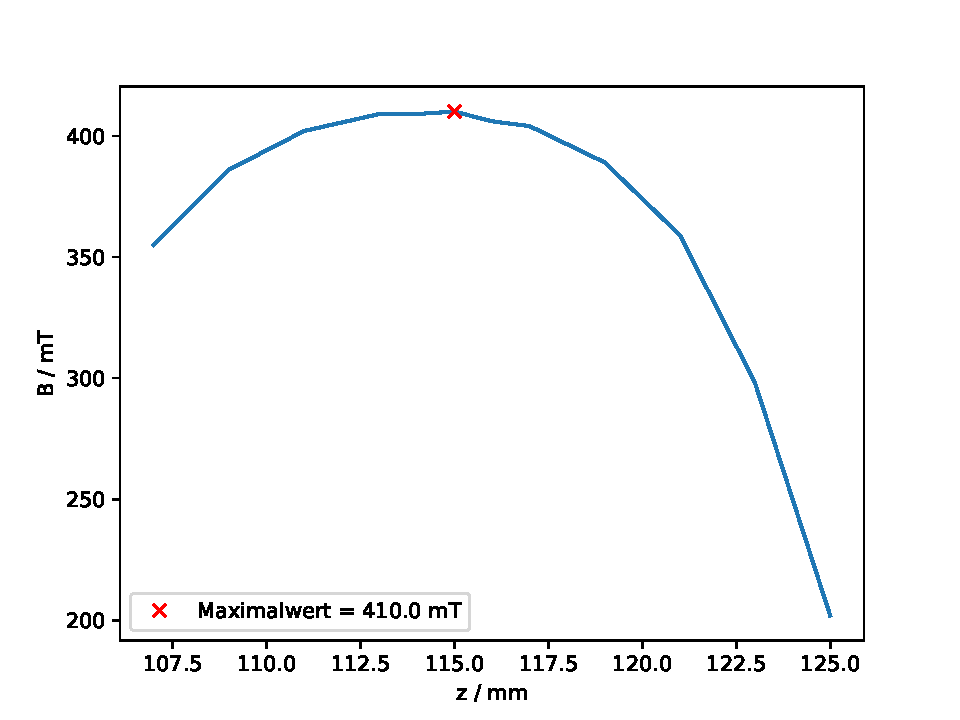
\includegraphics[width = \textwidth, keepaspectratio]{figure/BFeld_plot.pdf}
  \caption{Graphische Darstellung der Messwerte für die Bestimmung der maximalen Feldstärke}
  \label{fig:Feldstärke}
\end{figure}
\FloatBarrier
Der Maximale Wert liegt bei $\SI{410}{\milli\tesla}$. 
\subsection{Bestimmung der effektiven Masse}
Für die Bestimmung der effektiven Masse wird der Drehwinkel der Polarisationsebene in Abhängigkeit der Wellenlänge gemessen.
Diese Daten werden für zwei n-dotierte und eine reine Probe aufgenommen. Da die Proben unterschiedlich dick sind, wird 
der Drehwinkel auf die Dicke der Probe normiert.
Die Messwerte sind in Tablle \ref{tab:Drehwinkel} notiert.
\FloatBarrier
\begin{table}
  \centering
  \begin{tabular}{c c c c}
    \toprule
    $\lambda$ / \SI{}{\micro\meter}& $\theta_{\text{n-dotiert 1}}$ / $\frac{\SI{}{\radian}}{\SI{}{\micro\meter}}$& 
    $\theta_{\text{n-dotiert 2}}$ / $\frac{\SI{}{\radian}}{\SI{}{\micro\meter}}$&
    $\theta_{\text{rein}}$ / $\frac{\SI{}{\radian}}{\SI{}{\micro\meter}}$\\
    \midrule
    $\num{1.06} $&$\num{3.85e-4}$&$\num{1.57e-4}$&$\num{0.80e-4}$\\
    $\num{1.29} $&$\num{2.02e-4}$&$\num{1.25e-4}$&$\num{0.59e-4}$\\
    $\num{1.45} $&$\num{0.41e-4}$&$\num{1.22e-4}$&$\num{0.45e-4}$\\
    $\num{1.72} $&$\num{0.42e-4}$&$\num{1.31e-4}$&$\num{0.34e-4}$\\
    $\num{1.96} $&$\num{1.27e-4}$&$\num{1.45e-4}$&$\num{0.24e-4}$\\
    $\num{2.156}$&$\num{0.96e-4}$&$\num{1.63e-4}$&$\num{0.19e-4}$\\
    $\num{2.34} $&$\num{1.64e-4}$&$\num{1.75e-4}$&$\num{0.17e-4}$\\
    $\num{2.51} $&$\num{3.54e-4}$&$\num{2.05e-4}$&$\num{0.12e-4}$\\
    $\num{2.65} $&$\num{1.09e-4}$&$\num{1.84e-4}$&$\num{0.19e-4}$\\
    \bottomrule
  \end{tabular}
  \caption{Normierter Drehwinkel in Abhängigkeit der Wellenlänge. Die Dicken der Probe sind: Probe 1 $d=\SI{1360}{\micro\meter}$,
  Probe 2 $d=\SI{1296}{\micro\meter}$, reine Probe $d=\SI{5110}{\micro\meter}$.}
  \label{tab:Drehwinkel}
\end{table}
\FloatBarrier
Die Daten aus Tabelle \ref{tab:Drehwinkel} werden in Abbildung \ref{fig:Drehwinkel_1} und \ref{fig:Drehwinkel_2} 
dargestellt.
\FloatBarrier
\begin{figure}
  \centering
  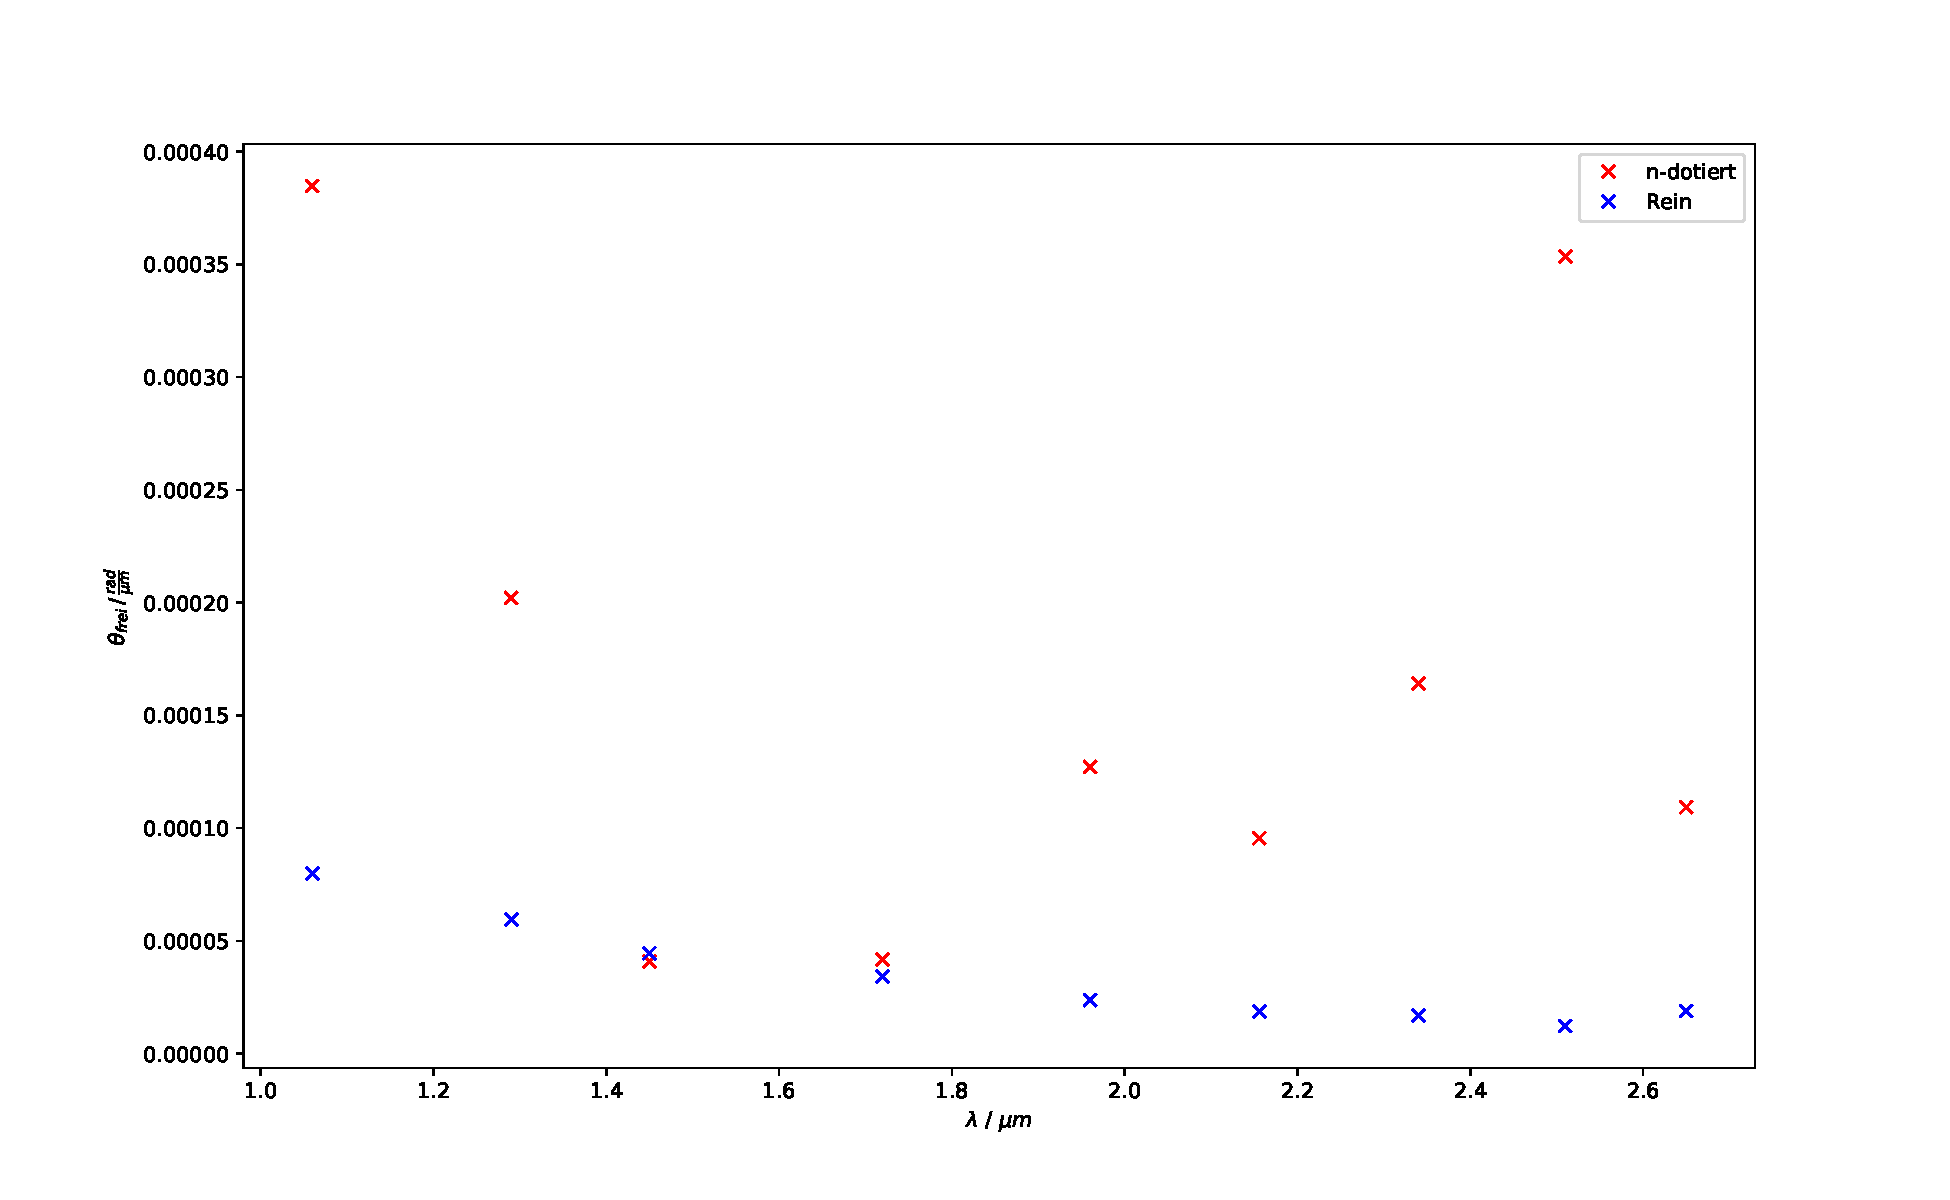
\includegraphics[width = \textwidth,keepaspectratio]{figure/Theta1_plot.pdf}
  \caption{Graphische Darstellung der normierten Drehwinkel, in Abhängigkeit der Wellenlänge, von der Probe 1 mit einer Dicke von $d=\SI{1360}{\micro\meter}$ und 
  der reinen Probe.}
  \label{fig:Drehwinkel_1}
\end{figure}
\begin{figure}
  \centering
  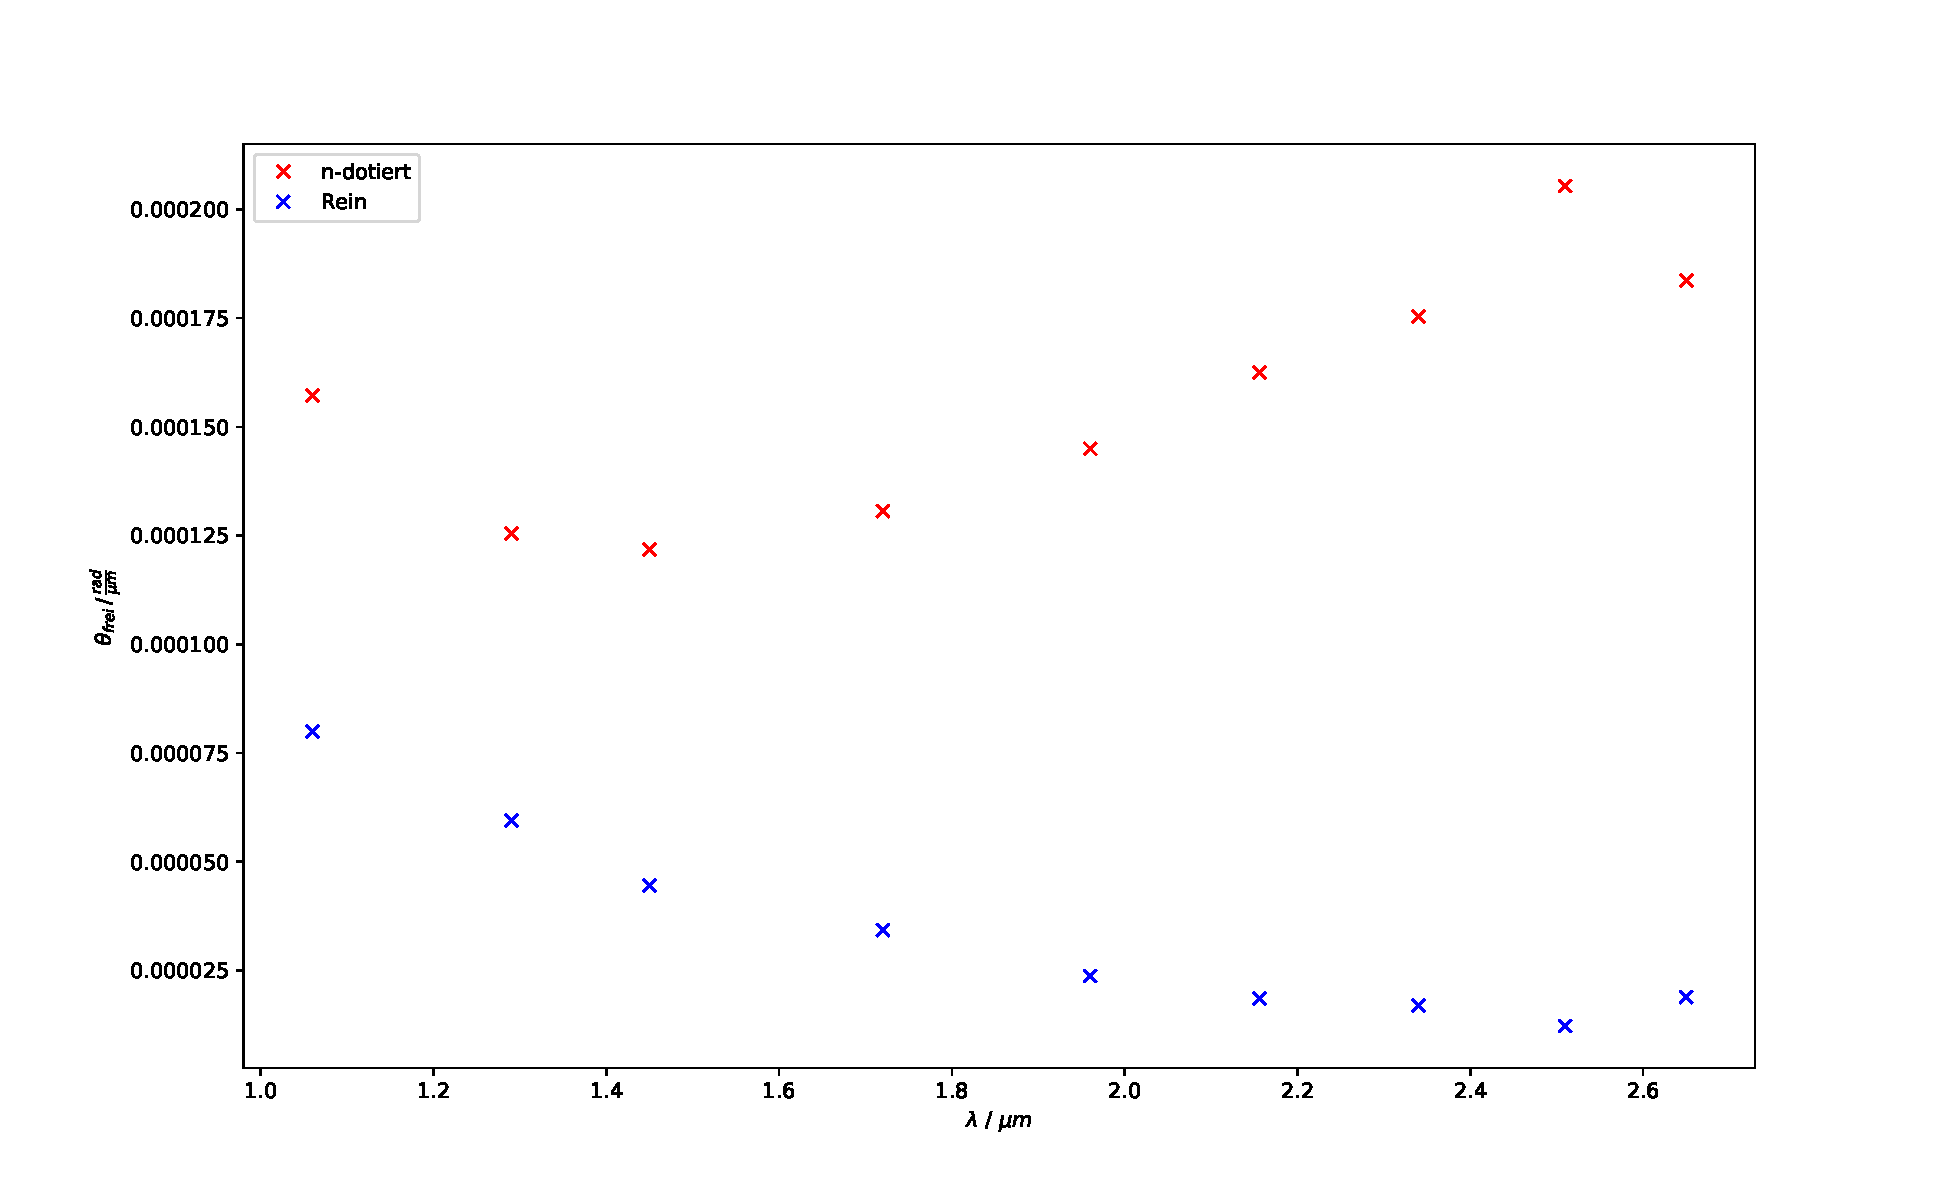
\includegraphics[width = \textwidth,keepaspectratio]{figure/Theta2_plot.pdf}
  \caption{Graphische Darstellung der normierten Drehwinkel, in Abhängigkeit der Wellenlänge, von der Probe 2 mit einer Dicke von $d=\SI{1296}{\micro\meter}$ und 
  der reinen Probe.}
  \label{fig:Drehwinkel_2}
\end{figure}
\FloatBarrier
Um die  Effektive Masse der Leitungselektronen bestimmen zu können, wird die Differenz der normierten Drehwinkel ermittelt
und gegen das Quadrat der Wellenlänge aufgetragen. Die Differenzen sind in Tablle \ref{tab:Differenzen} aufgelistet.
\FloatBarrier
\begin{table}
  \centering
  \begin{tabular}{c c c}
    \toprule
    $\lambda^2$ / \SI{}{\micro\meter\square}&$\Delta_{\text{1}}$ / $\frac{\SI{}{\radian}}{\SI{}{\micro\meter}}$&$\Delta_{\text{2}}$ / $\frac{\SI{}{\radian}}{\SI{}{\micro\meter}}$\\
    \midrule 
    $\num{1.1}$&$\num{3.05e-4}$&$ \num{0.77e-4}$\\
    $\num{1.7}$&$\num{1.43e-4}$&$ \num{0.66e-4}$\\
    $\num{2.1}$&$\num{-0.04e-4}$&$\num{0.77e-4}$\\
    $\num{3.0}$&$\num{0.07e-4}$&$ \num{0.96e-4}$\\
    $\num{3.8}$&$\num{1.04e-4}$&$ \num{1.21e-4}$\\
    $\num{4.6}$&$\num{0.77e-4}$&$ \num{1.44e-4}$\\
    $\num{5.5}$&$\num{1.47e-4}$&$ \num{1.58e-4}$\\
    $\num{6.3}$&$\num{3.41e-4}$&$ \num{1.93e-4}$\\
    $\num{7.0}$&$\num{0.9e-4}$&$  \num{1.65e-4}$\\
    \bottomrule
  \end{tabular}
  \caption{Messwerte zur Bestimmung der effektiven Masse von Ladungselektronen.}
  \label{tab:Differenzen}
\end{table}
\FloatBarrier
Die Daten werden gegeneinander aufgetragen und die Funktion \eqref{eq:fit} wird an die Daten gefittet.
\begin{equation}
  \label{eq:fit}
  \theta_{\text{frei}} = f(\lambda^2) = a\cdot \lambda^2
\end{equation}
Die Daten aus Tablle \ref{tab:Differenzen} und der dazugehörige Fit sind in den Abbildungen \ref{fig:fit1} und \ref{fig:fit2} 
dargestellt.
\FloatBarrier
\begin{figure}
  \centering
  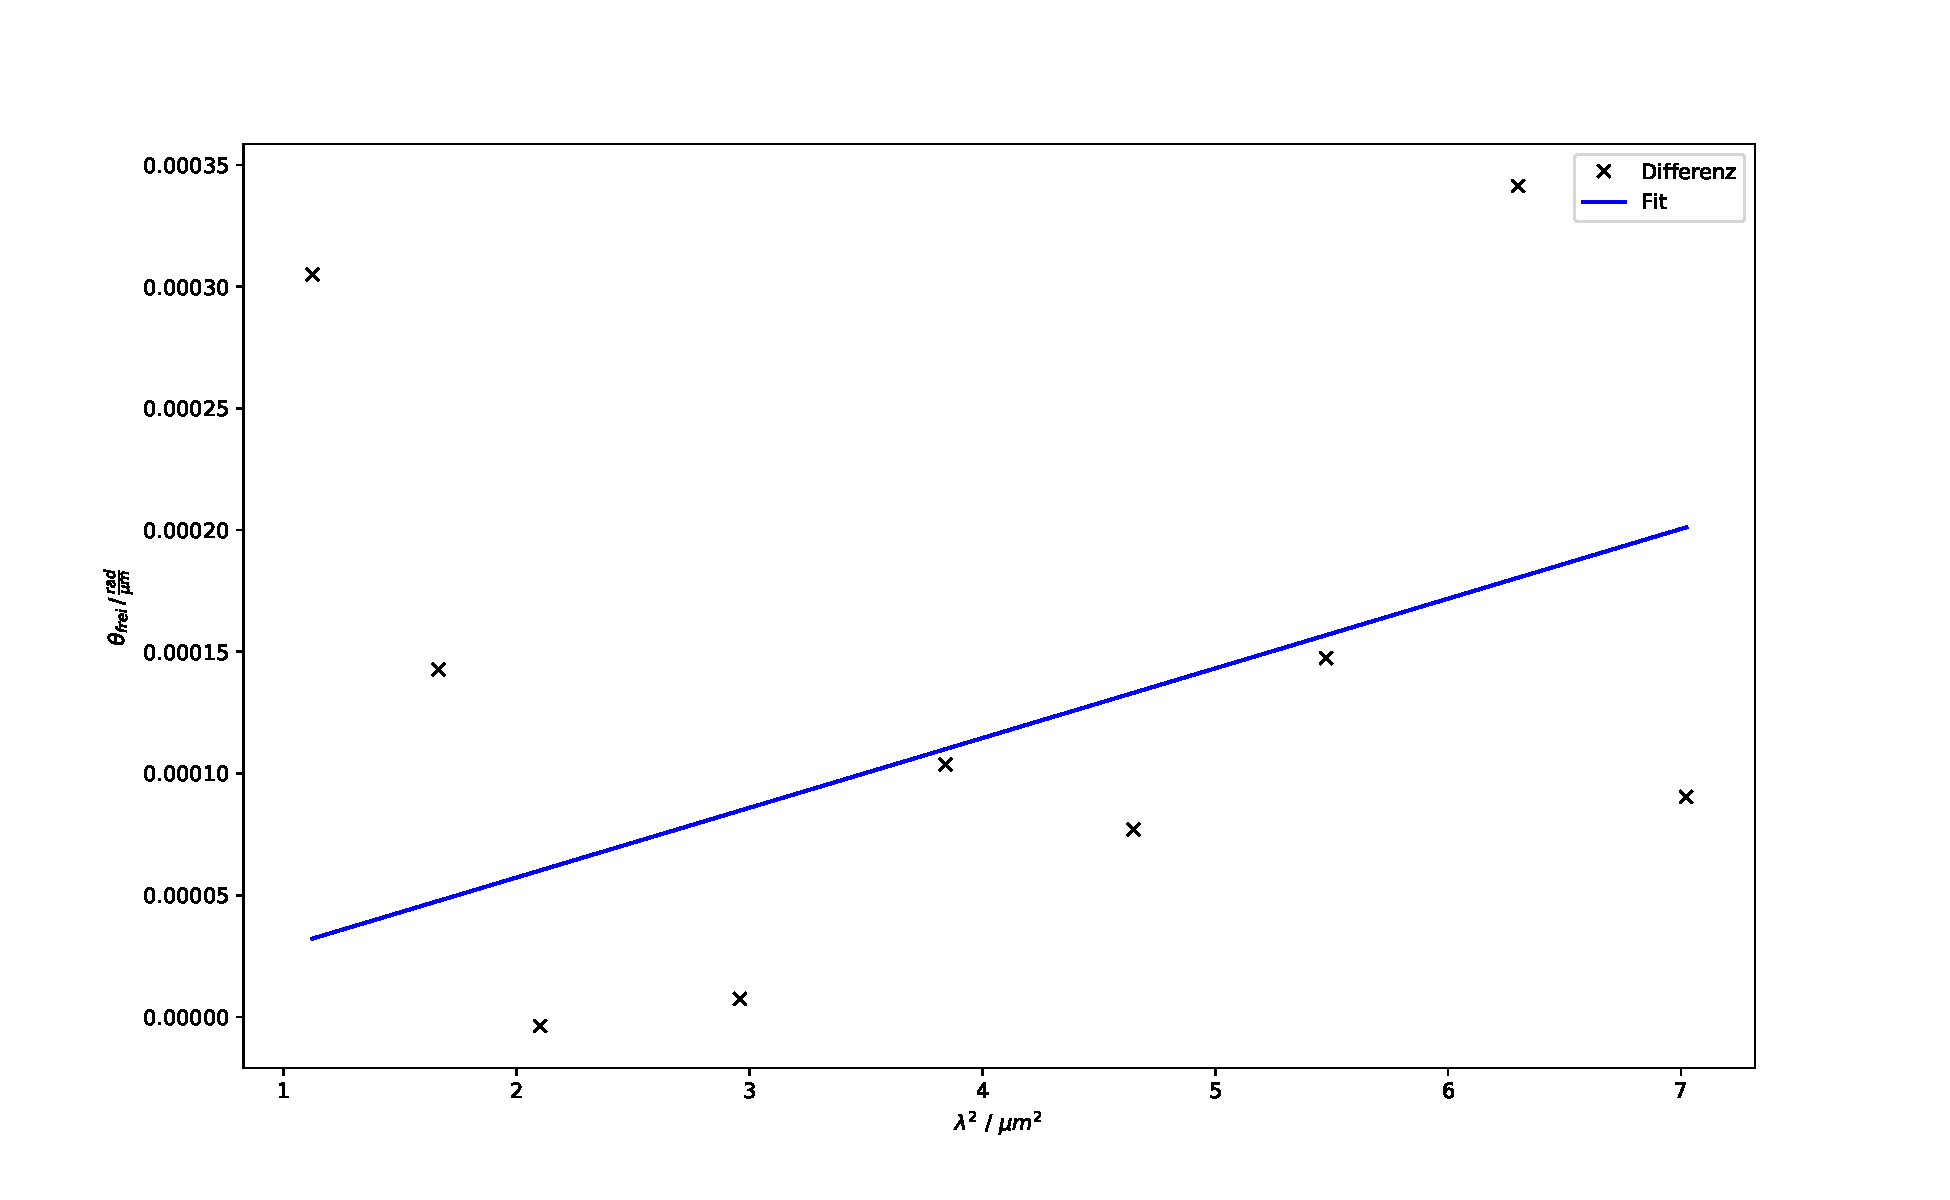
\includegraphics[width = \textwidth]{figure/Theta1_diff_plot.pdf}
  \caption{Plot zur Bestimmung der effektiven Masse mittels Probe 1}
  \label{fig:fit1}
\end{figure}
\begin{figure}
  \centering
  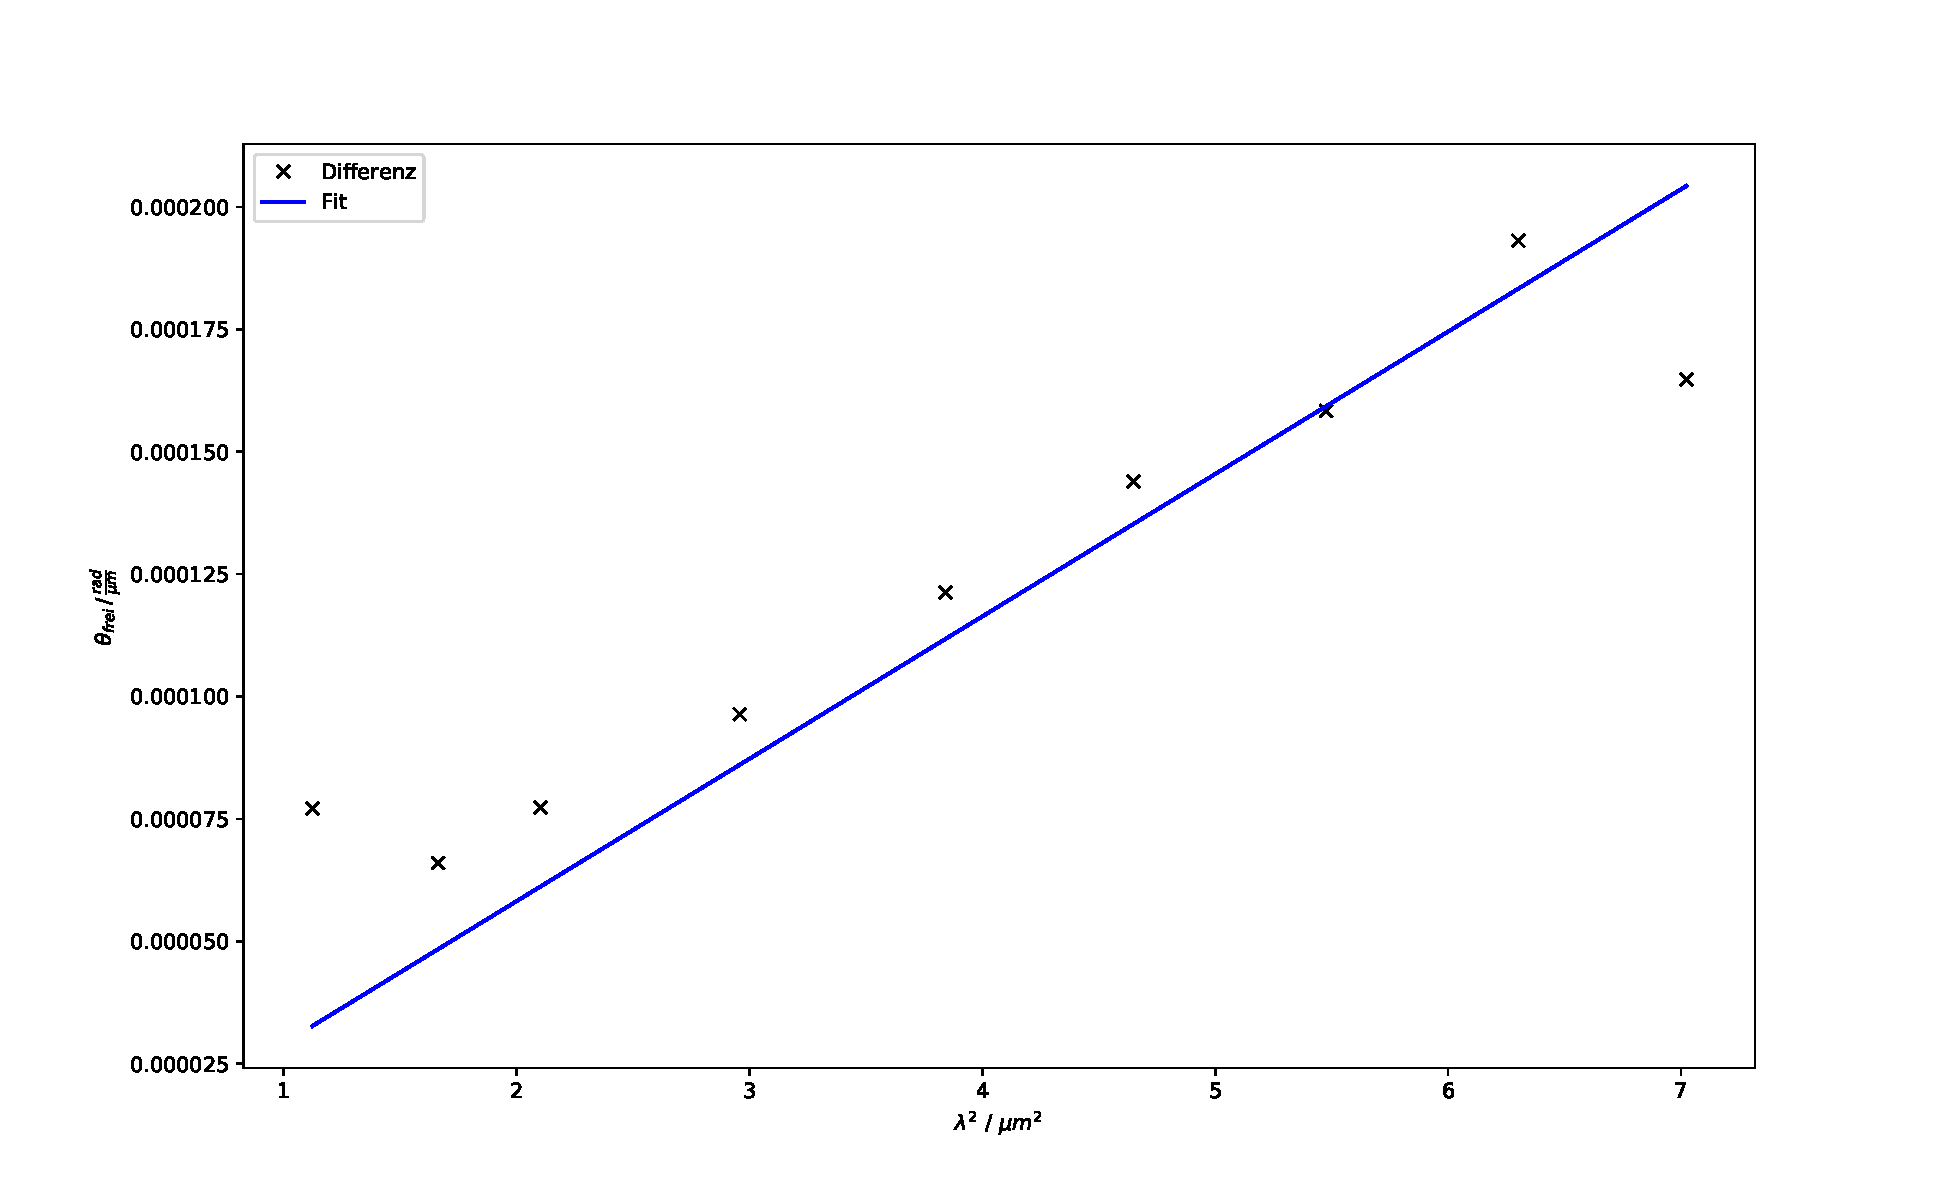
\includegraphics[width = \textwidth]{figure/Theta2_diff_plot.pdf}
  \caption{Plot zur Bestimmung der effektiven Masse mittels Probe 2}
  \label{fig:fit2}
\end{figure}
\FloatBarrier
Die Fitparameter der beiden Funktionen sind:
\begin{align*}
  a_{\text{1}} =& \num{3(1)e13}  \,\frac{\SI{}{\radian}}{\SI{}{\cubic\meter}}\\
  a_{\text{2}} =& \num{2.9(1)e13}\,\frac{\SI{}{\radian}}{\SI{}{\cubic\meter}}.
\end{align*}
Der Wert $a$ kann in die folgende Gleichung eingesetzt werden, um die effektive Masse zu bestimmen.
\begin{align*}
  &\theta_{\text{frei}} = \frac{\symup{e}_0^3}{8\pi^2\epsilon_0\symup{c}^3 \left(m^*\right)^2}\lambda^2\frac{NB}{n}\\
  &\implies \left(m^*\right)=\sqrt{\frac{\symup{e}_0^3}{8\pi^2\epsilon_0\symup{c}^3} \left(\frac{\lambda^2}{\theta_{\text{frei}}}\right)\frac{NB}{n} }\\
  &\implies \left(m^*\right)=\sqrt{\frac{\symup{e}_0^3}{8\pi^2\epsilon_0\symup{c}^3} \left(\frac{1}{a}\right)\frac{NB}{n} }
\end{align*}
Die effektive Masse beträgt:
\begin{equation*}
  m^*_1 = \SI{3.2(6)e-32}{\kilo\gram}\qquad m^*_2 = \SI{4.9(1)e-32}{\kilo\gram}
\end{equation*}